\subsubsection*{(b) Análise da interpretabilidade dos modelos}

Para cada um dos gráficos gerados pelos códigos abaixo, explicamos o que está sendo mostrado, como isso se relaciona com as previsões do modelo em questão e se é possível interpretar com facilidade o que está acontecendo.

\textbf{(i) Parâmetros do Naive Bayes}

\begin{lstlisting}[language=Python]
nb_params = {}
for i in range(10):
    nb_params[i] = np.exp(nb.feature_log_prob_[i])

plot_digits(nb_params)
\end{lstlisting}

\begin{figure}[H]
    \centering
    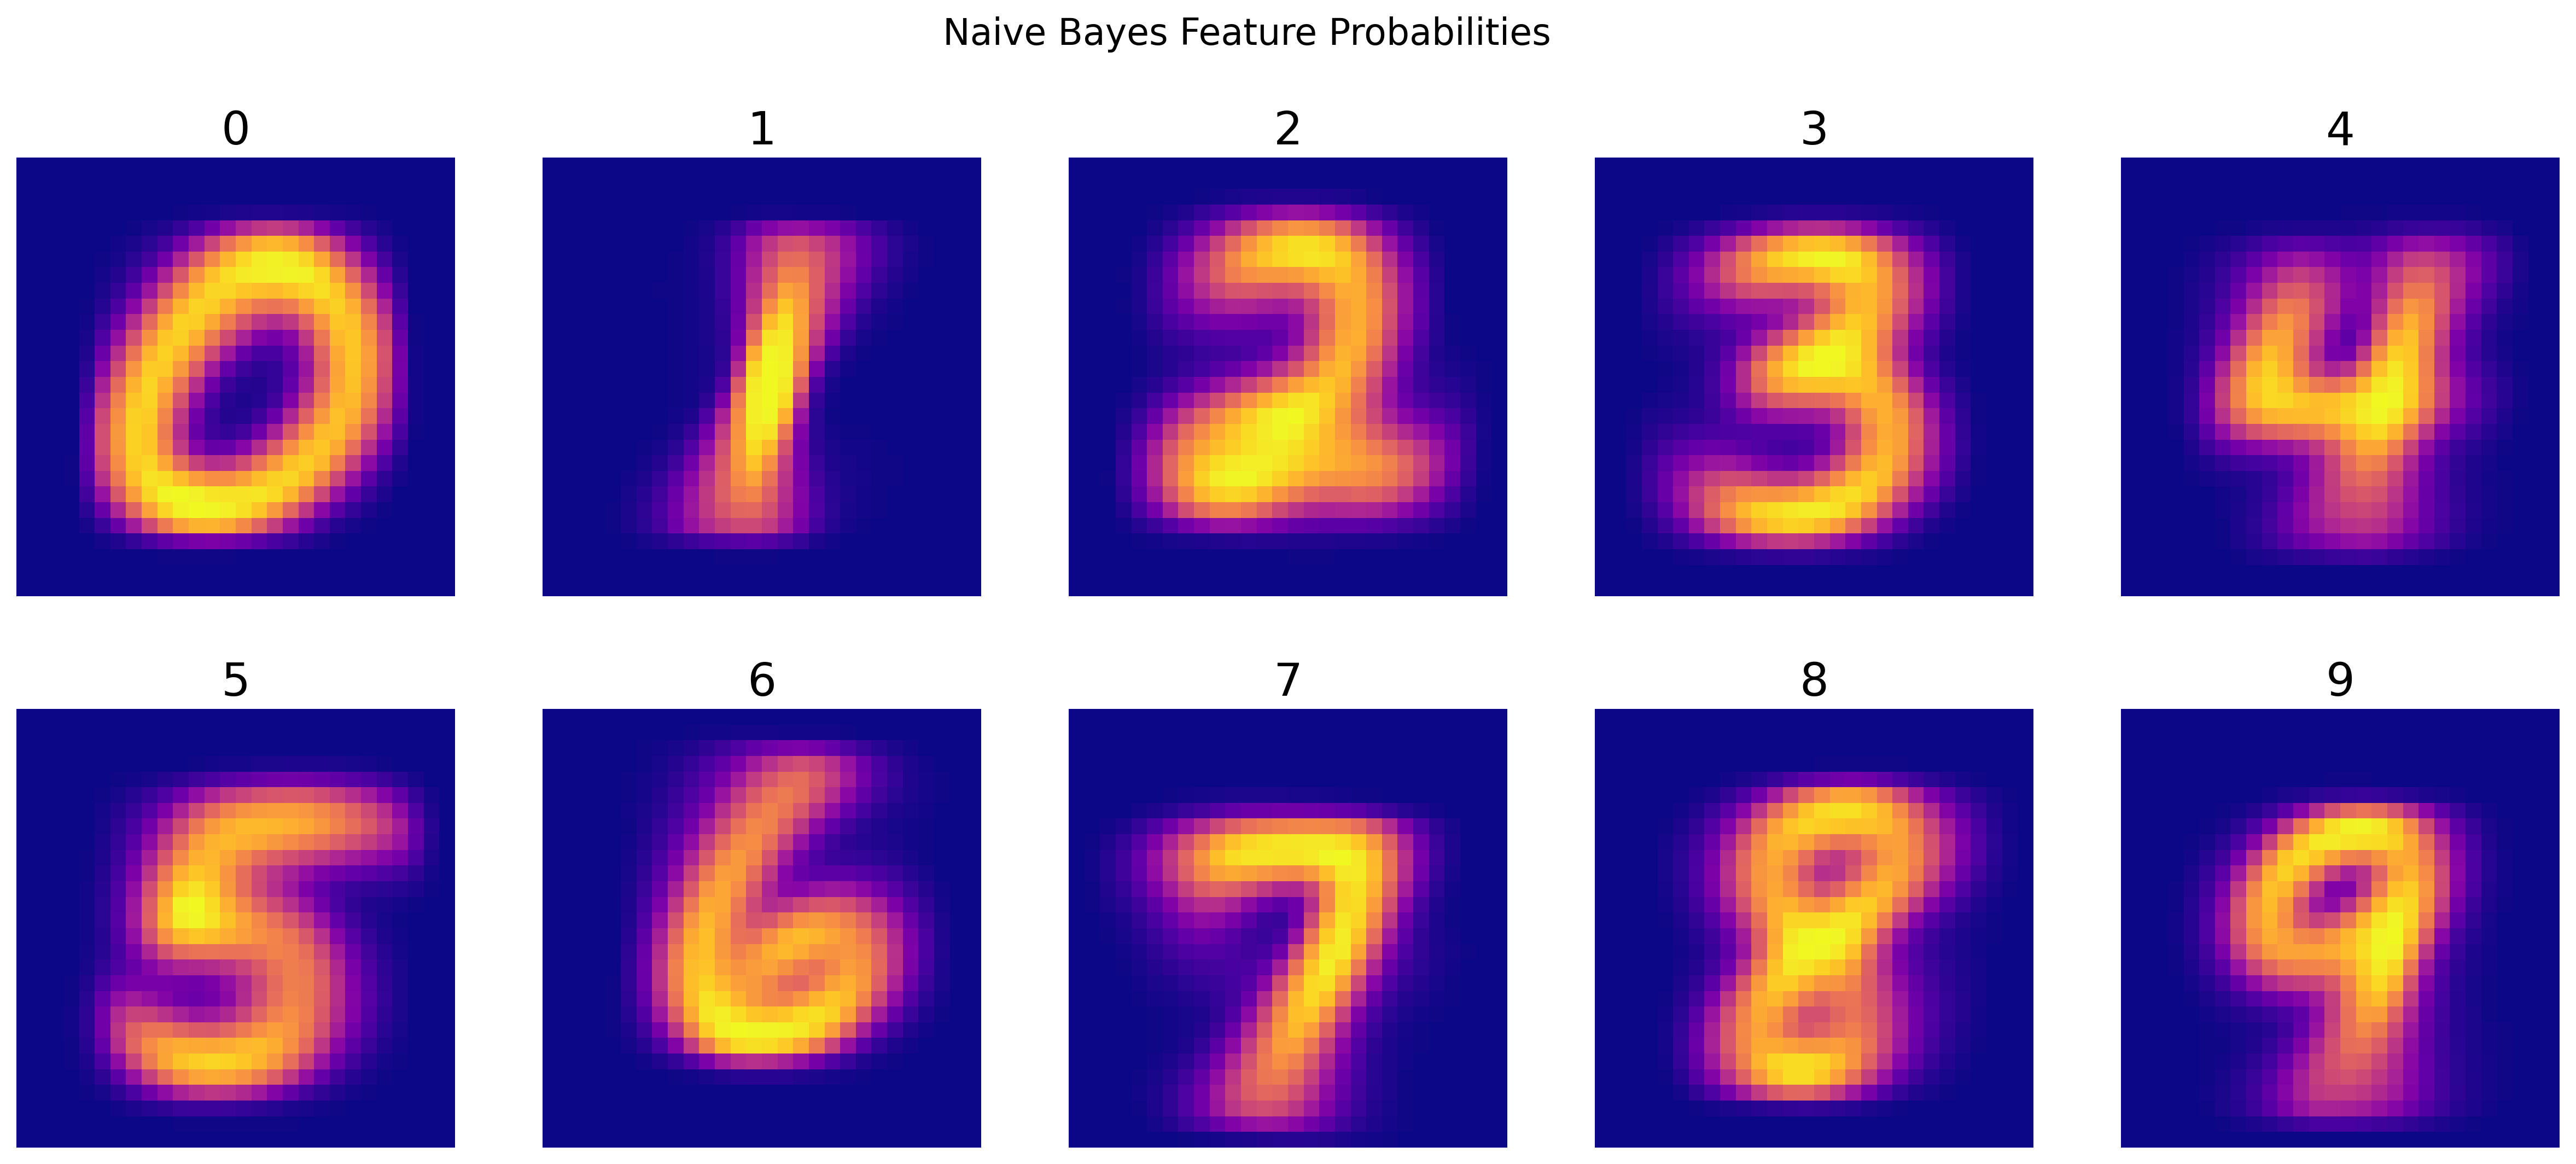
\includegraphics[width=0.8\textwidth]{../figures/3/naive_bayes_params.png}
    \caption{Probabilidades dos pixels para cada classe no modelo Naive Bayes}
    \label{fig:nb_params}
\end{figure}

Cada imagem representa a probabilidade dos pixels da imagem pertencerem à respectiva classe, sendo que valores altos indicam pixels recorrentes para a classe. O produto entre este vetor e a entrada indicará a probabilidade da entrada ser pertencente à classe e será utilizada para classificação. A interpretação da imagem é simples e permite a reconstituição do dígito ao qual a classe referencia.

\textbf{(ii) Parâmetros do LDA}

\begin{lstlisting}[language=Python]
lda_params = {}
for i in range(10):
    lda_params[i] = lda.means_[i]

plot_digits(lda_params)
\end{lstlisting}

\begin{figure}[H]
    \centering
    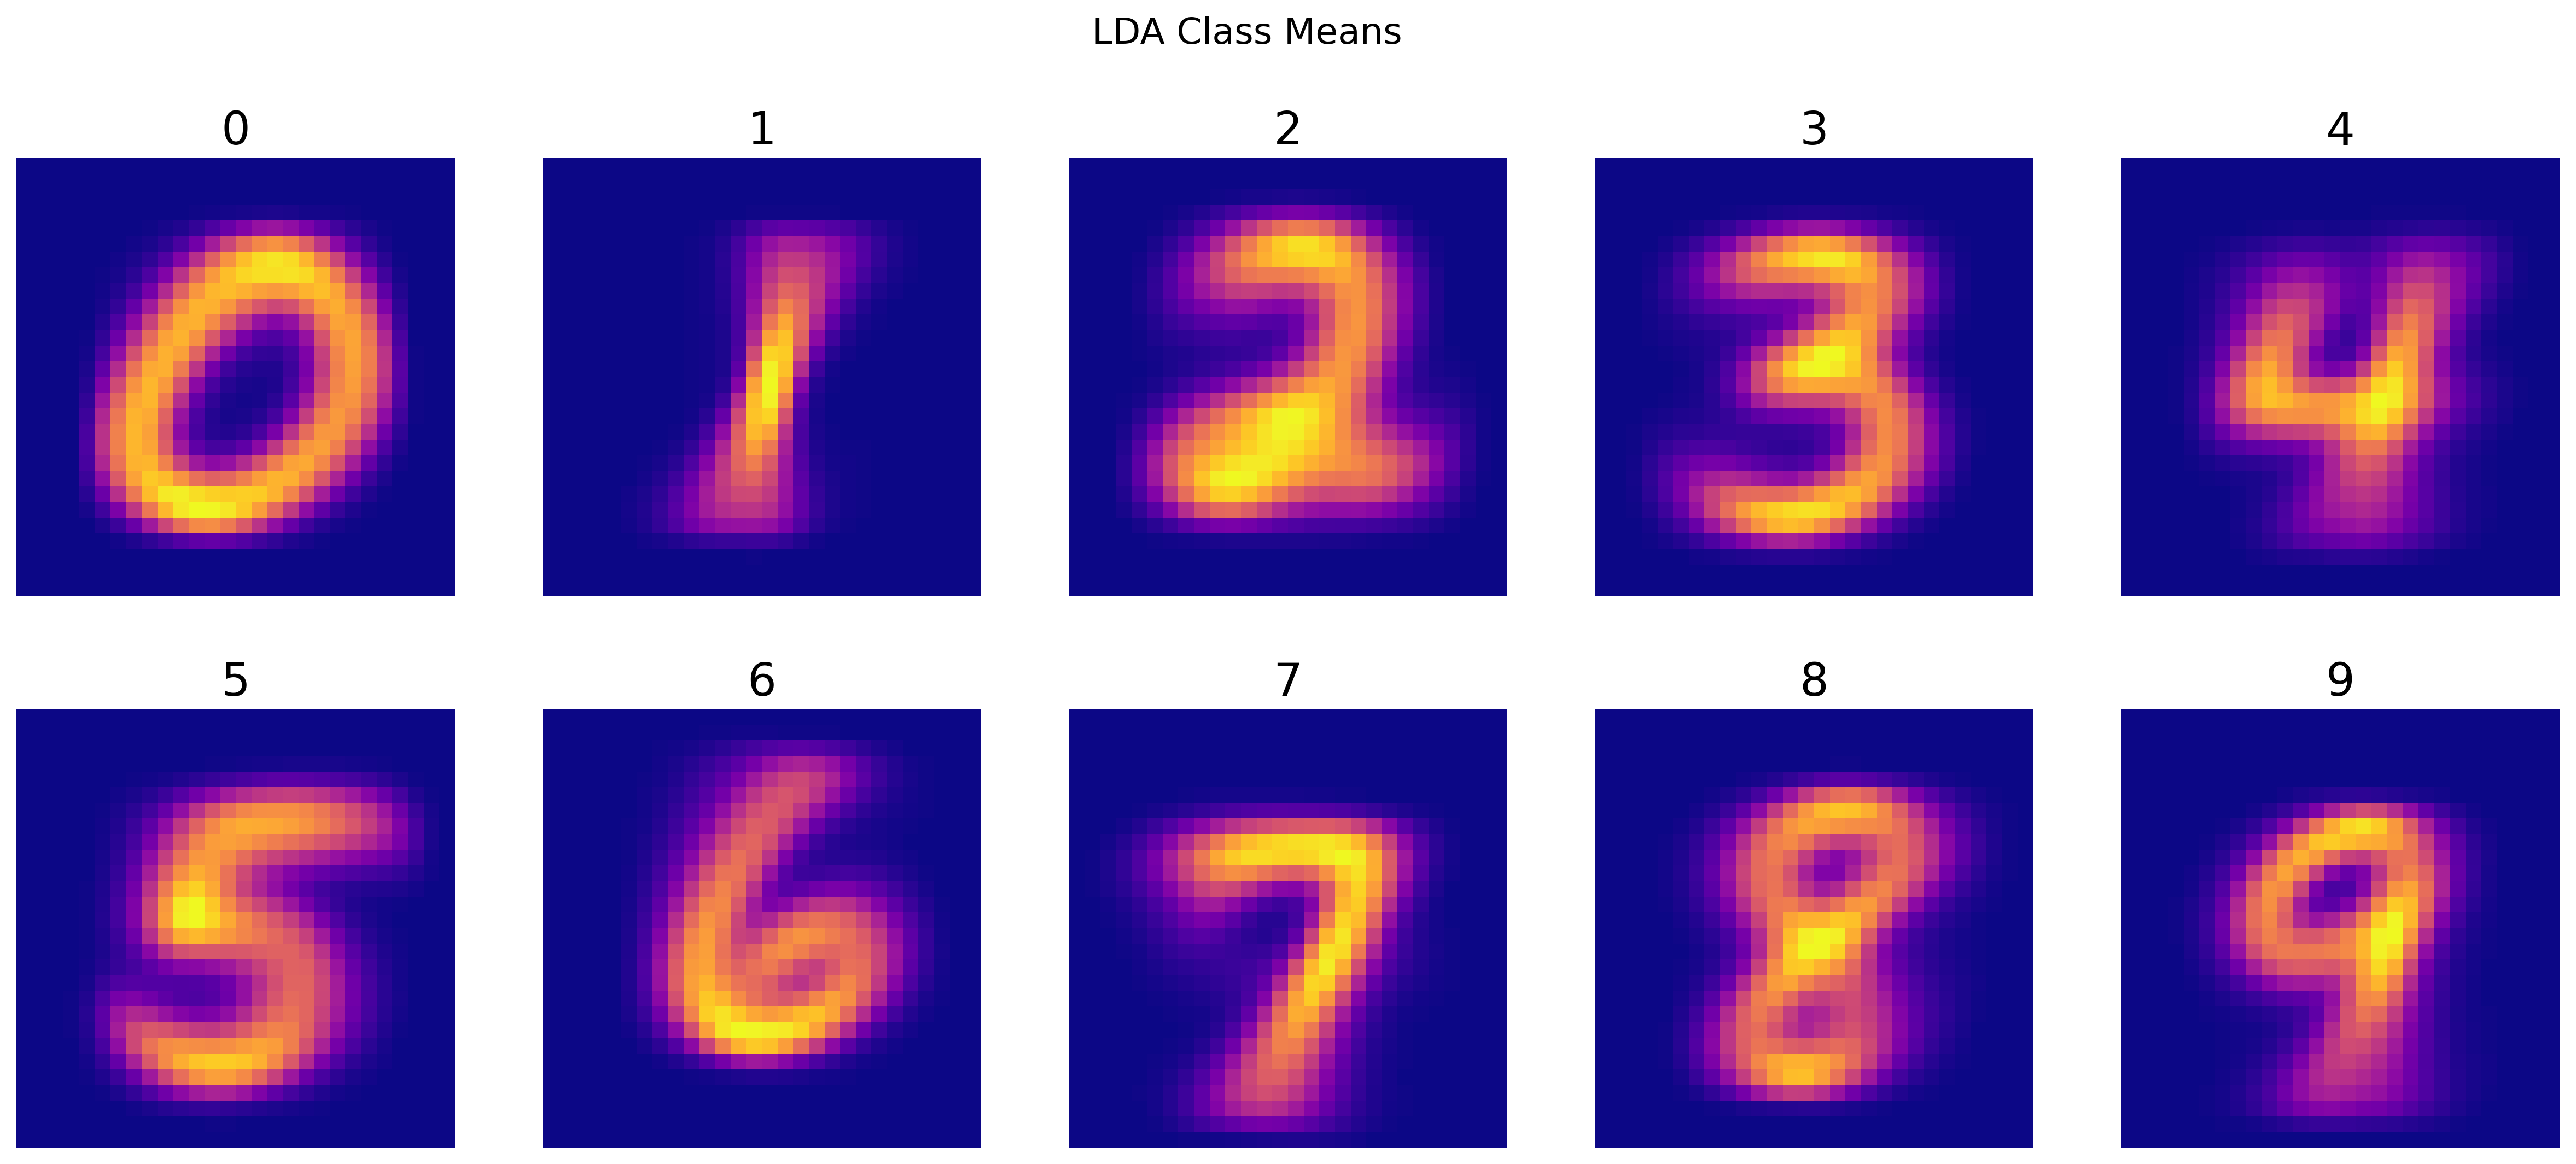
\includegraphics[width=0.8\textwidth]{../figures/3/lda_params.png}
    \caption{Médias das classes no modelo LDA}
    \label{fig:lda_means}
\end{figure}

Cada uma das imagens é a média da respectiva classe no espaço de entrada. Essa imagem seria equivalente a uma amostra média, ponto central em relação às demais amostras da classe. As previsões do modelo baseiam-se em uma métrica de similaridade da entrada em relação a cada uma dessas médias. É possível interpretar com facilidade a classe relacionada a cada imagem.

\textbf{(iii) Parâmetros da Regressão Logística}

\begin{lstlisting}[language=Python]
log_reg_params = {}
for i in range(10):
    log_reg_params[i] = lr.coef_[i]

plot_digits(log_reg_params)
\end{lstlisting}

\begin{figure}[H]
    \centering
    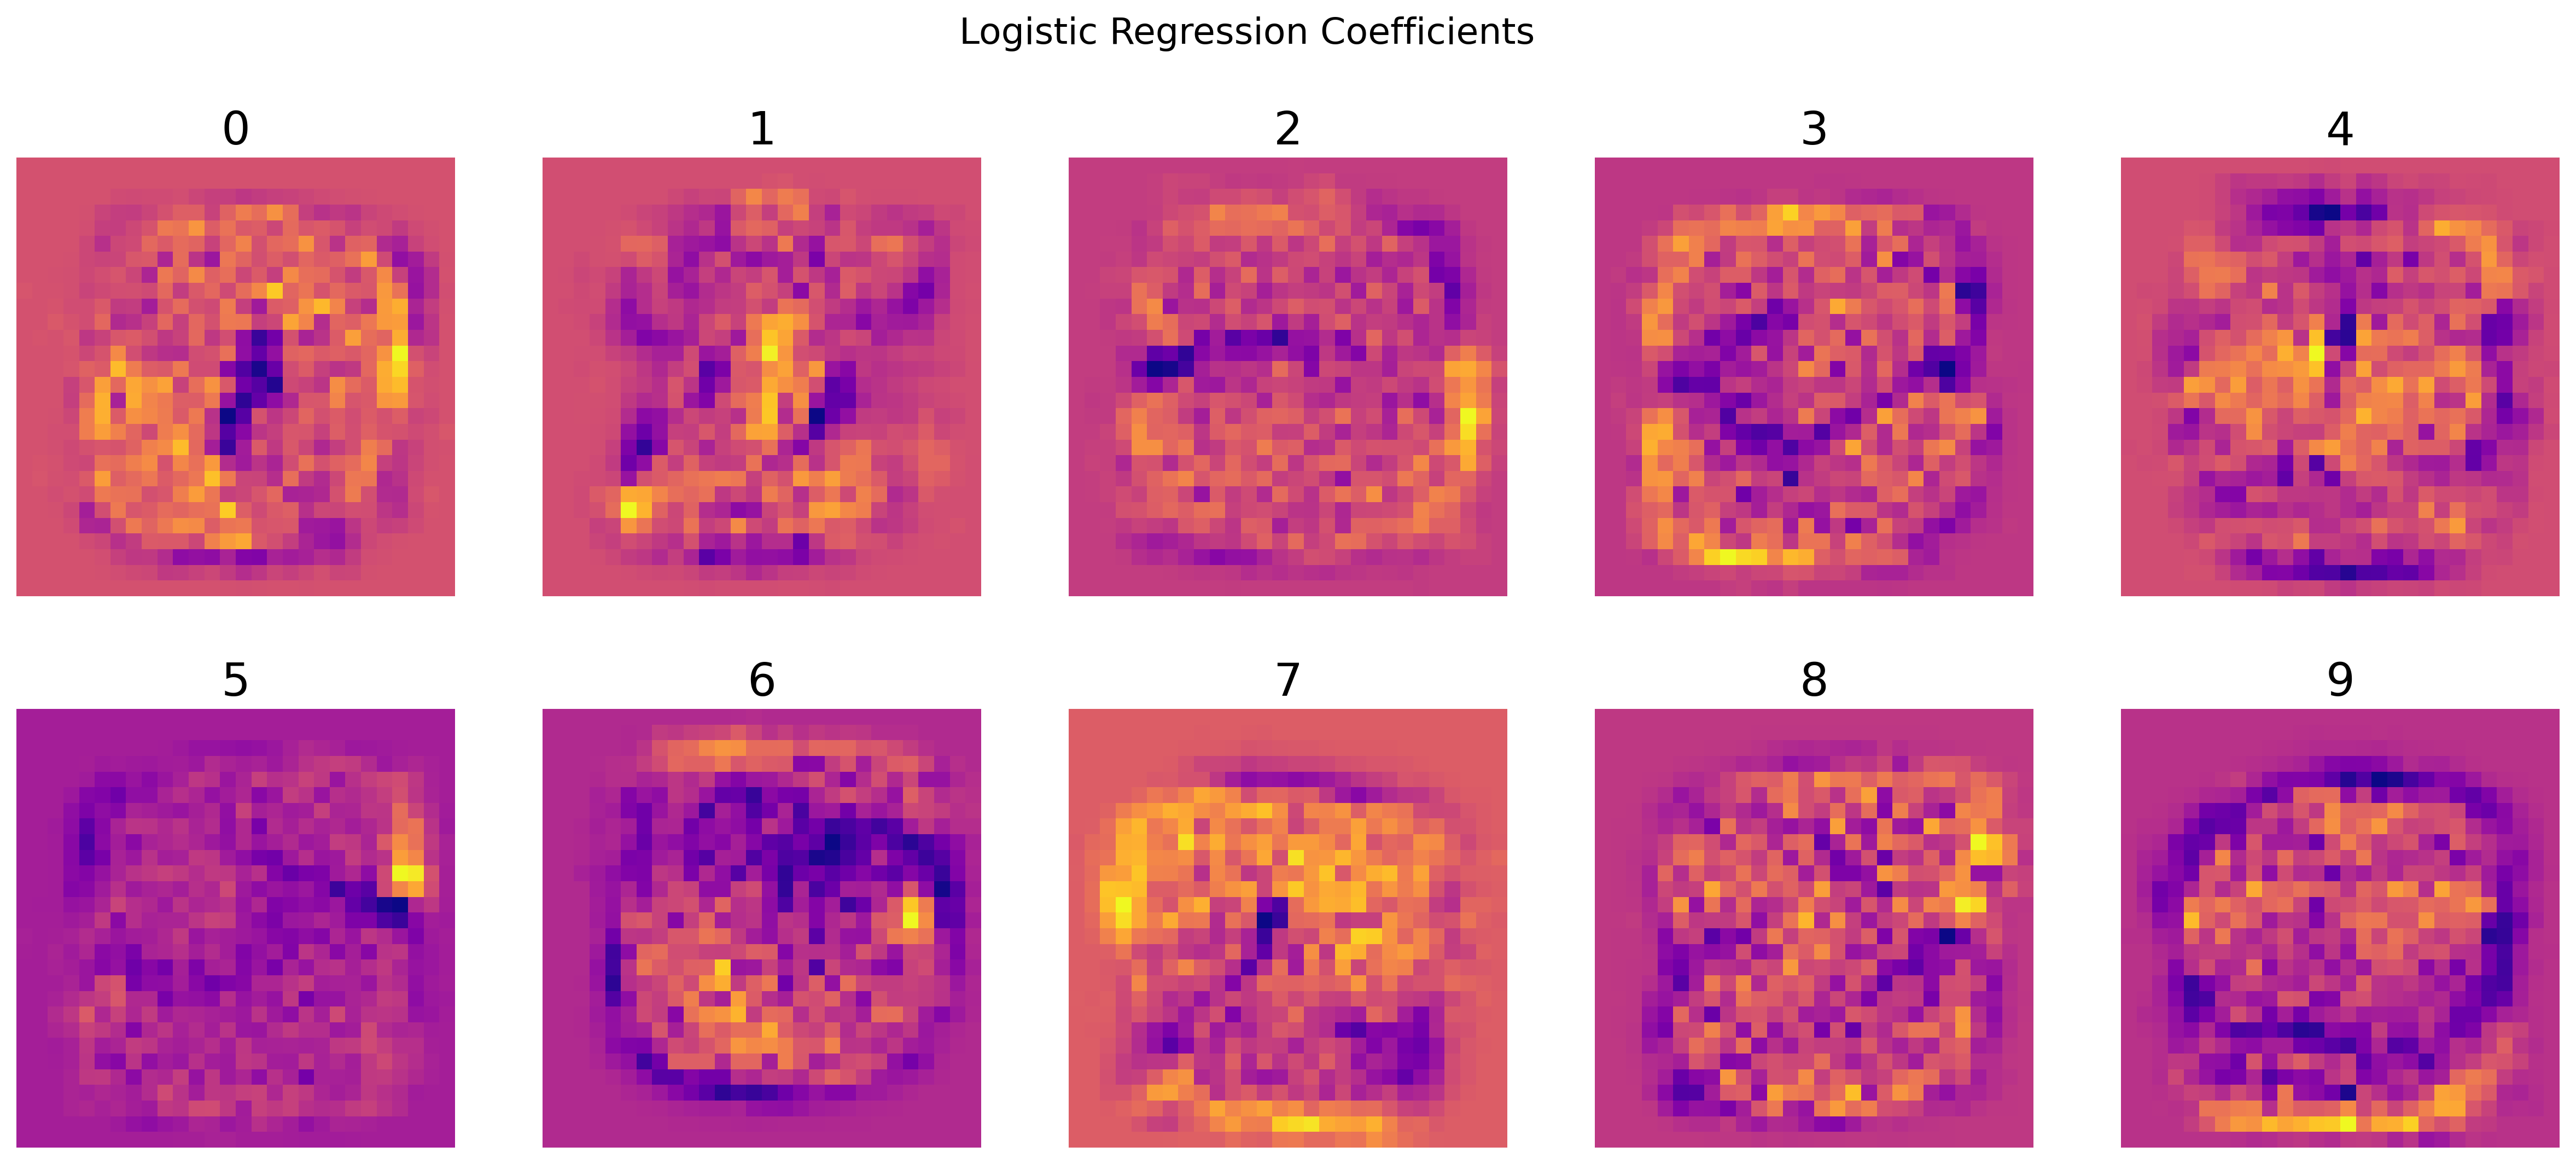
\includegraphics[width=0.8\textwidth]{../figures/3/logistic_regression_params.png}
    \caption{Coeficientes do modelo de Regressão Logística}
    \label{fig:lr_coefs}
\end{figure}

A imagem representa o coeficiente da rede. Ao multiplicarmos pela entrada, teremos o logaritmo da probabilidade da amostra pertencer à classe sobre a probabilidade dela pertencer à classe de referência. A imagem mostrada é a resposta do modelo a uma matriz de 1's. Isso pode ser interpretado como a contribuição de cada pixel para a probabilidade final. Ainda mantemos uma interpretação válida de cada classe por meio da imagem, apesar de menos clara caso comparemos com as imagens dos modelos anteriores.

\textbf{(iv) Importância das features no Random Forest}

\begin{lstlisting}[language=Python]
rf_params = rf.feature_importances_.reshape(28, 28)

plt.axis("off")
plt.imshow(rf_params, cmap="plasma")
\end{lstlisting}

\begin{figure}[H]
    \centering
    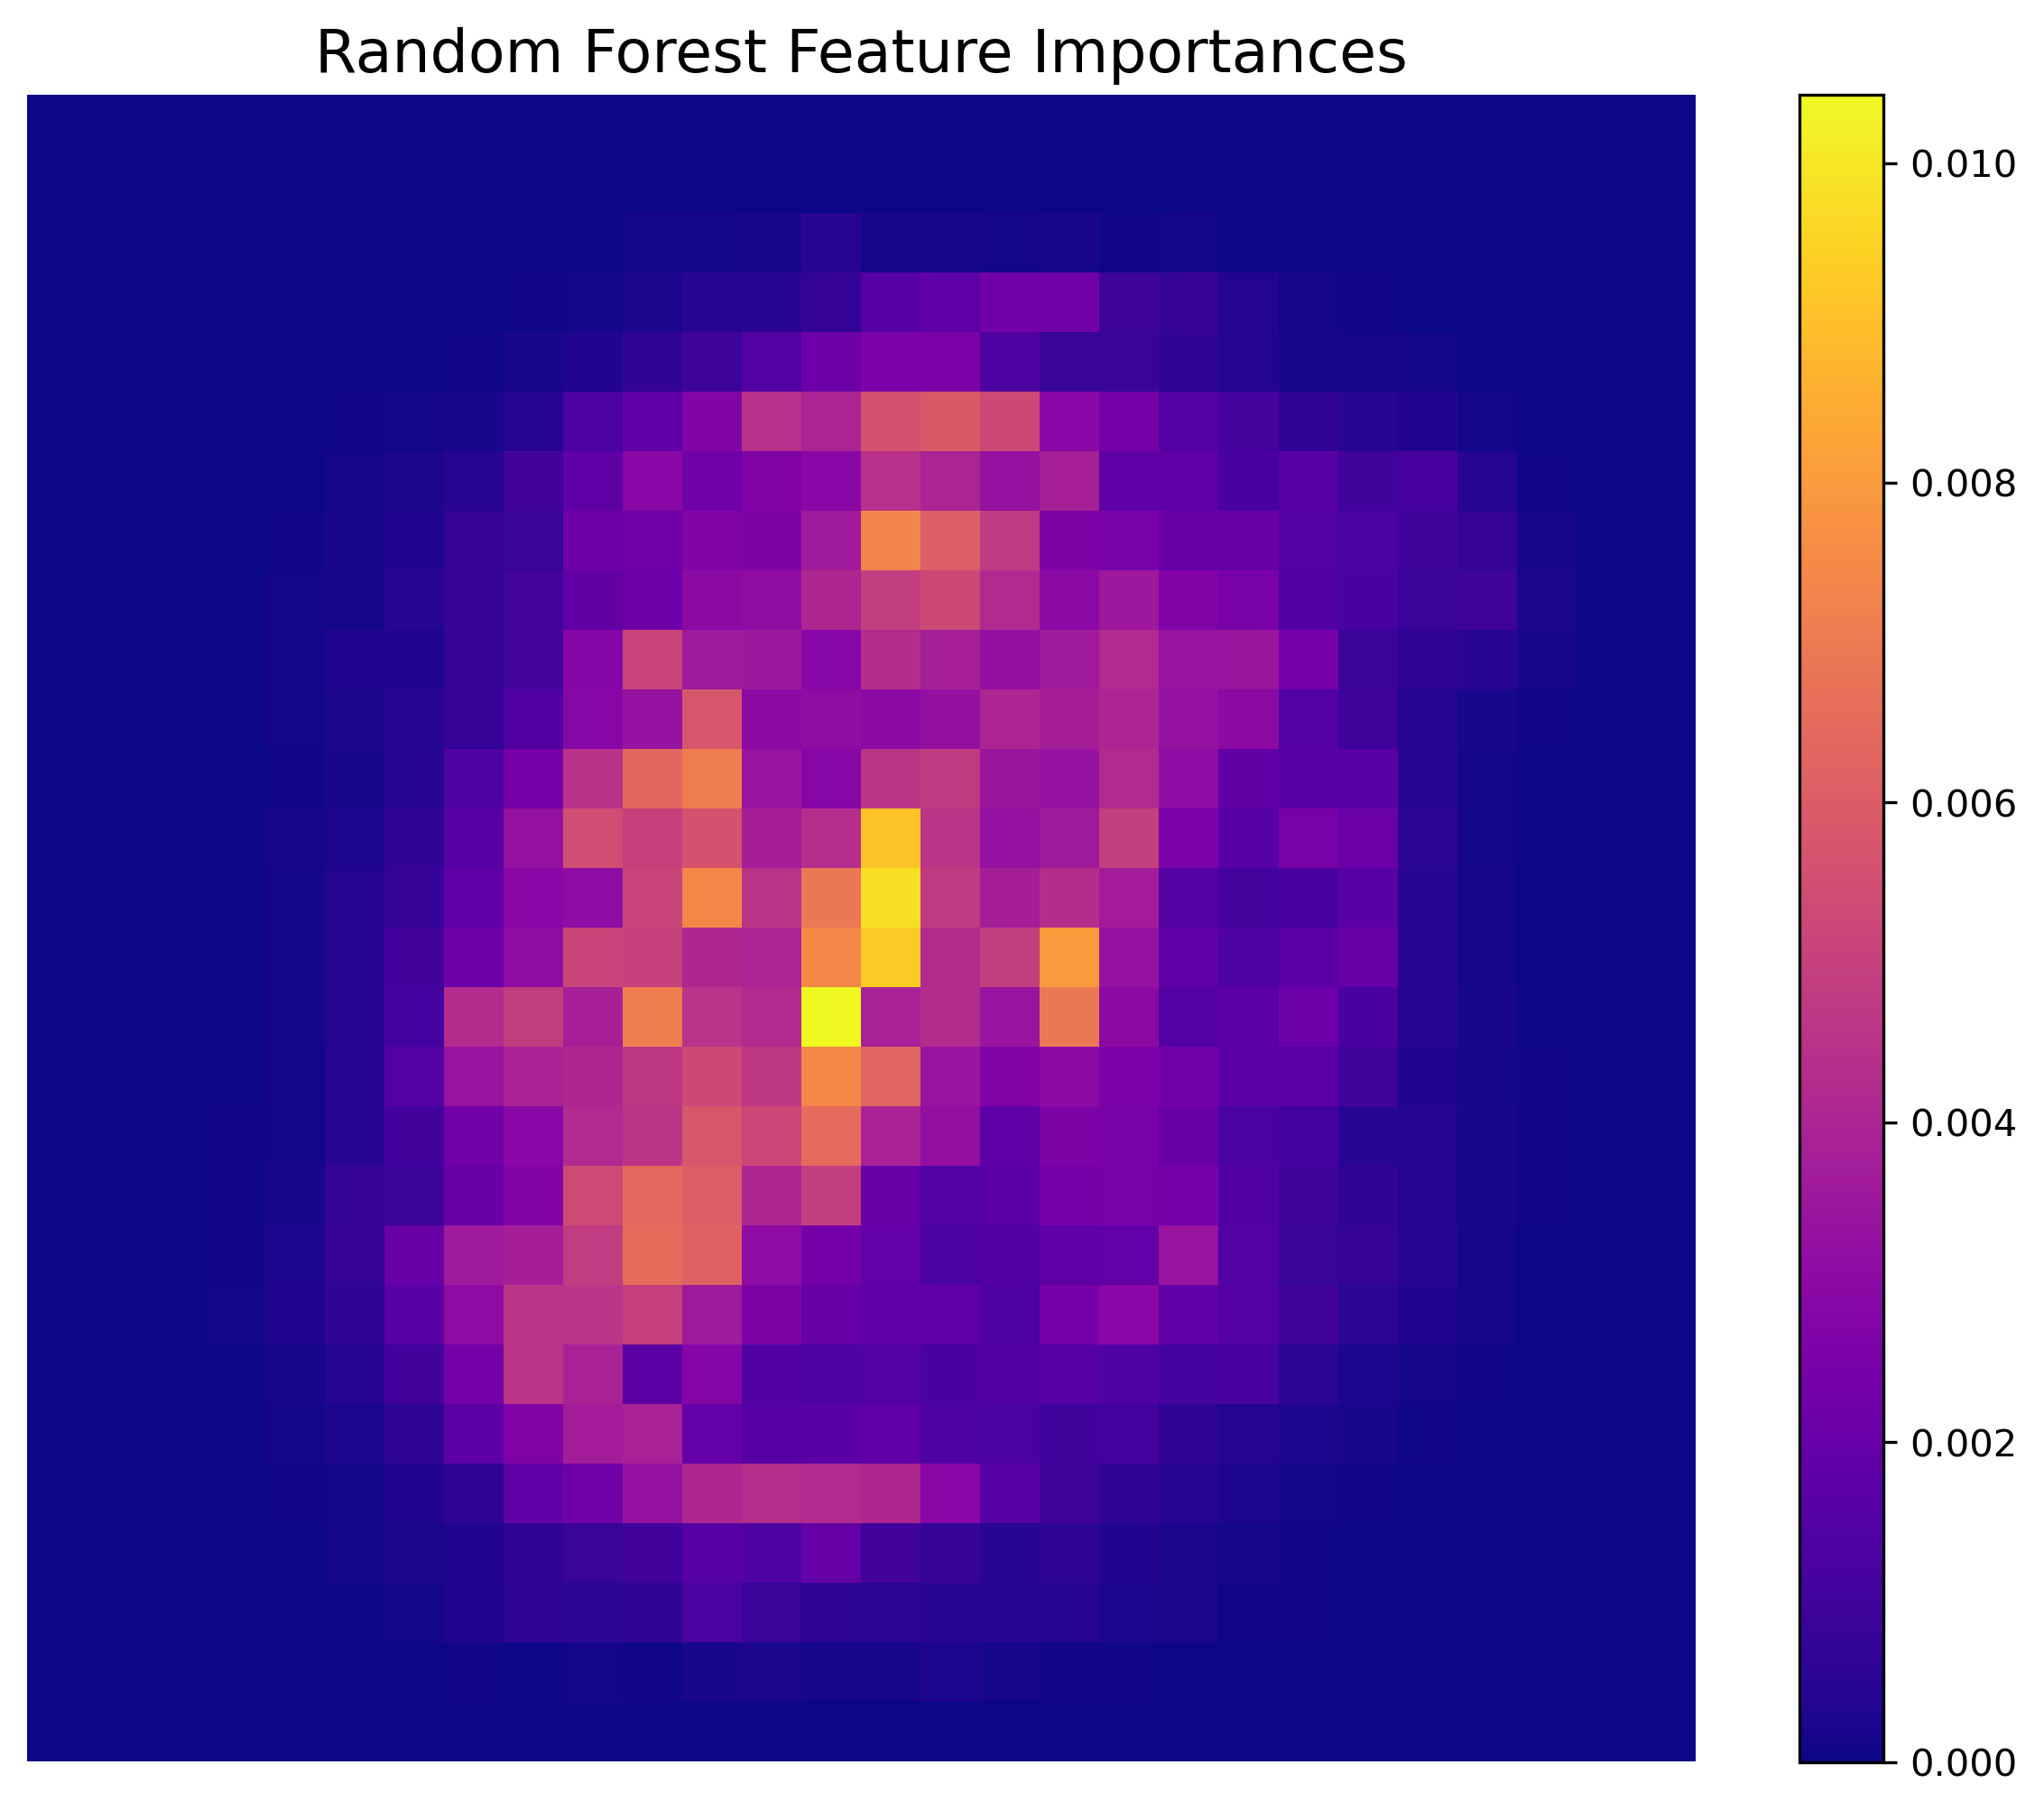
\includegraphics[width=0.6\textwidth]{../figures/3/random_forest_feature_importance.png}
    \caption{Importância das features no modelo Random Forest}
    \label{fig:rf_importance}
\end{figure}

A imagem representa a importância de cada pixel para o modelo, baseada na média do decaimento de uma métrica de impureza, no caso, o coeficiente de Gini. Valores altos indicam que aquela feature foi capaz de auxiliar na distinção entre as classes. Nesse caso, perde-se a interpretação individual das classes, entretanto ainda está clara qual a região mais importante para a classificação.

\textbf{(v) Parâmetros da Rede Neural}

\textbf{(v.a) Pesos da camada de entrada para a camada oculta}

\begin{lstlisting}[language=Python]
nn_params_1 = {}
for i in range(100):
    nn_params_1[i] = nn.coefs_[0][:, i]

indexes = list(range(100))

plot_digits(
    nn_params_1,
    n_rows=10,
    n_cols=10,
    fig_shape=(100, 100),
    indexes=indexes,
    img_shape=(28, 28),
    labels=None,
)
\end{lstlisting}

\begin{figure}[H]
    \centering
    \includegraphics[width=0.9\textwidth]{../figures/3/neural_network_input_hidden_weights.png}
    \caption{Pesos da camada de entrada para a camada oculta na Rede Neural}
    \label{fig:nn_layer1}
\end{figure}

Cada imagem representa os pesos que ligam a entrada a cada um dos neurônios da camada oculta. Eles são a transformação linear da entrada antes da primeira função de ativação e podem ser interpretados como parte de uma engenharia de features. A interpretabilidade já se perdeu completamente, tanto pela alta quantidade de neurônios quanto pela dificuldade de encontrar valor semântico em cada transformação.

\textbf{(v.b) Pesos da camada oculta para a camada de saída}

\begin{lstlisting}[language=Python]
nn_params_2 = {}
for i in range(10):
    nn_params_2[i] = nn.coefs_[1][:, i]

plot_digits(
    nn_params_2, n_rows=2, n_cols=5, fig_shape=(20, 8), img_shape=(10, 10)
)
\end{lstlisting}

\begin{figure}[H]
    \centering
    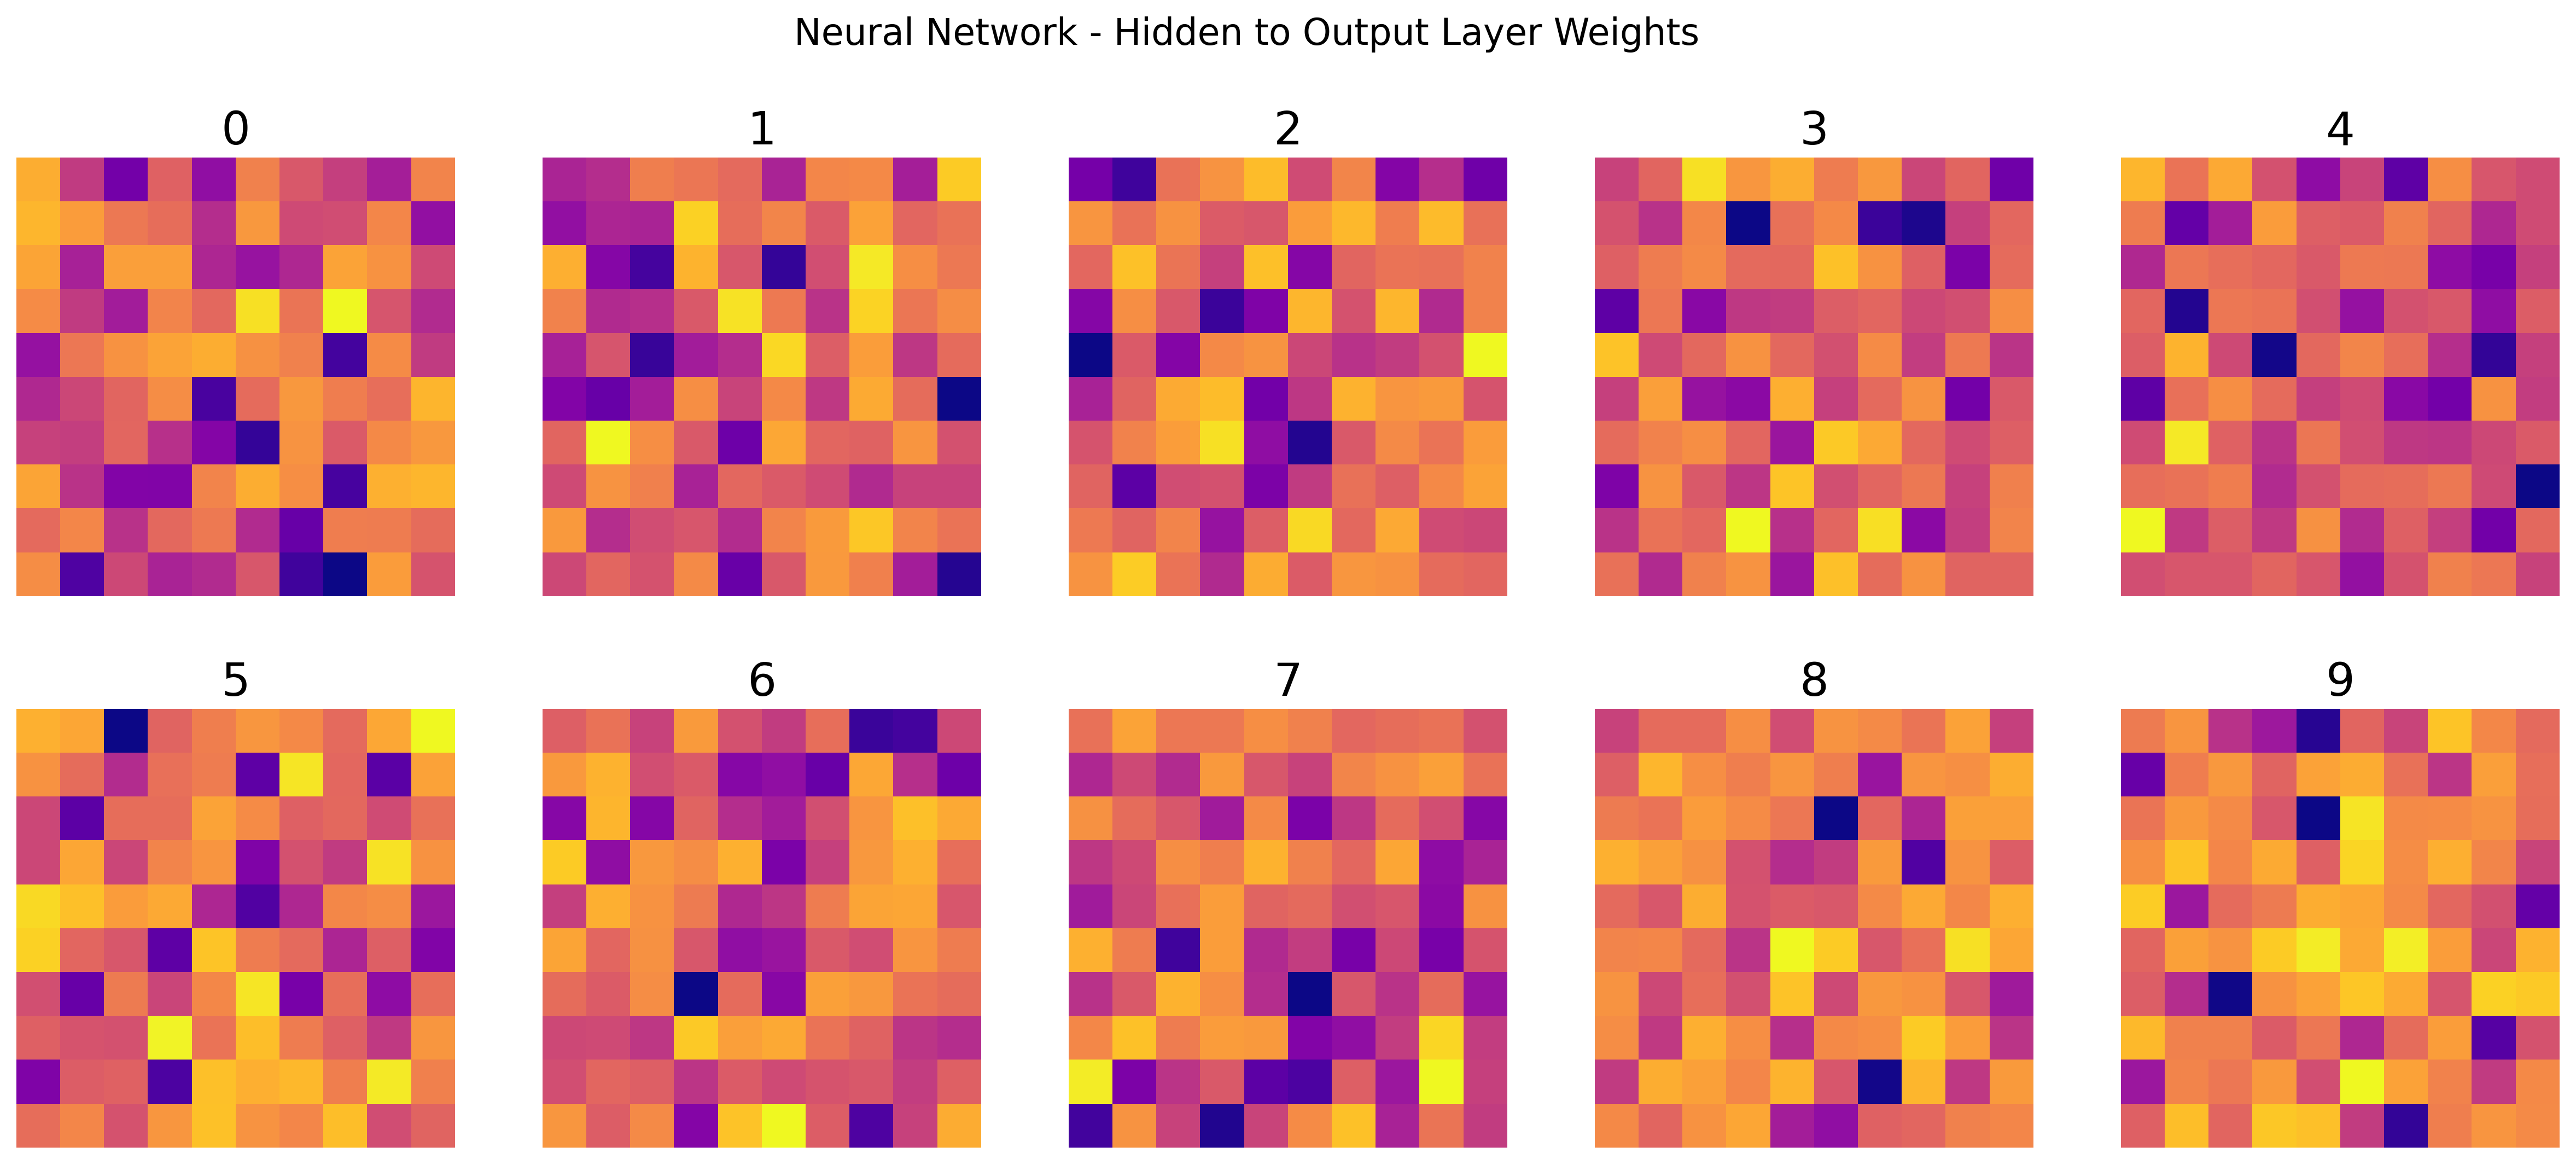
\includegraphics[width=0.8\textwidth]{../figures/3/neural_network_hidden_output_weights.png}
    \caption{Pesos da camada oculta para a camada de saída na Rede Neural}
    \label{fig:nn_layer2}
\end{figure}

Cada imagem representa os pesos que ligam a camada escondida da rede à camada de saída, em que uma regressão logística será realizada. Seria semelhante ao que ocorre no modelo de regressão logística do item anterior. Entretanto, como o espaço de features é a projeção da entrada na camada intermediária, a interpretação se perde, não podendo relacionar cada classe ao numeral correspondente.

